\documentclass{standalone}
\usepackage{ tikz }
\usetikzlibrary{shapes}
\usetikzlibrary{plotmarks}
\usepackage{ xparse }
\usepackage{../../../macros}

\begin{document}
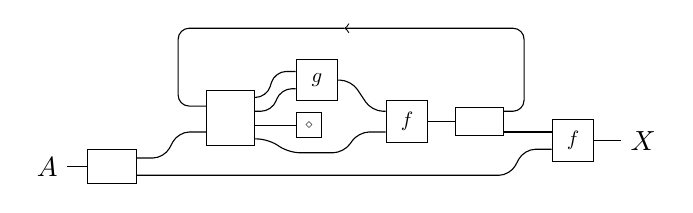
\begin{tikzpicture}[yscale=-1,x=1em,y=1.25em]
        
    \node [anchor=east] at (-3,1) {$A$};
    \draw (-3,1) -- (-2.25,1);
    \node[draw, minimum height = 1.25em, minimum width = 1.75em, anchor = east] at (-0.5,1){$\ccopy{}$};
    \draw [rounded corners] (-0.5,0.75) -- (0.5,0.75) -- (1,0) -- (2,0);
    \draw [rounded corners] (-0.5,1.25) -- (13,1.25) -- (13.5,0.5) -- (14.5,0.5);
    \node[draw, minimum height = 2em, minimum width = 1.75em, anchor = west] at (2,-0.4){$\ccopy{}$};
    \draw [rounded corners] (3.75,-1) -- (4.2,-1) -- (4.5,-1.75) -- (5.25,-1.75);
    \draw [rounded corners] (3.75,-0.6) -- (4.4,-0.6) -- (4.7,-1.25) -- (5.25,-1.25);
    \draw (3.75,-0.2) -- (5.25,-0.2);
    \draw [rounded corners] (3.75,0.2) -- (4.25, 0.2) -- (5,0.6) -- (7,0.6) -- (7.5,0) -- (8.5,0);
    \node[draw, minimum height = 1.5em, minimum width = 1.5em, anchor = west] at (5.25,-1.5){\scalebox{0.75}{$g$}};
    \node[draw, minimum height = 0.25em, minimum width = 0.25em, anchor = west] at (5.25,-0.2){\scalebox{0.5}{$\diamond$}};
    \draw [rounded corners] (6.75, -1.5) -- (7.25,-1.5) -- (8,-0.6) -- (8.5,-0.6);
    \node[draw, minimum height = 1.5em, minimum width = 1.5em, anchor = west] at (8.5,-0.3){\scalebox{0.75}{$f$}};
    \draw (10,-0.3) -- (11,-0.3);
    \node[draw, minimum height = 1em, minimum width = 1.75em, anchor = west] at (11,-0.3){$\ccopy{}$};
    \draw [rounded corners, ->] (12.75,-0.6) -- (13.5,-0.6) -- (13.5, -3) -- (7,-3);
    \draw [rounded corners] (7,-3) -- (1,-3) -- (1,-0.75) -- (2,-0.75);
    \draw (12.75, 0) -- (14.5,0);
    \node[draw, minimum height = 1.5em, minimum width = 1.5em, anchor = west] at (14.5,0.25){\scalebox{0.75}{$f$}};
    \node [anchor=west] at (17,0.25) {$X$};
    \draw (16,0.25) -- (17,0.25);

\end{tikzpicture}
\end{document}